\documentclass[conference]{IEEEtran}
\IEEEoverridecommandlockouts
% The preceding line is only needed to identify funding in the first footnote. If that is unneeded, please comment it out.
\usepackage{cite}
\usepackage{setspace}
\setstretch{1.387916}
\usepackage{amsmath,amssymb,amsfonts}
\usepackage{algorithmic}
\usepackage{graphicx}
\usepackage{textcomp}
\usepackage{xcolor}
\usepackage{hyperref}
\usepackage{wasysym}
\usepackage{caption2}
\newcommand{\BibTeX}{\textrm{B \kern -.05em \textsc{i \kern -.025em b} \kern -.08em
T \kern -.1667em \lower .7ex \hbox{E} \kern -.125emX}}
\begin{document}

    \title{KMeans Kernel Classifier\\
    {\footnotesize \textsuperscript {}Course: Math Behind ML }
    }

    \author{\IEEEauthorblockN{Karthik Kurugodu}
    \IEEEauthorblockA{\textit{B.Tech Mathematics and Computing} \\
    {Indian Institute of Technology Hyderabad}\\
    ma20btech11008@iith.ac.in}
    \and
    \IEEEauthorblockN{Nikhil Kongara}
    \IEEEauthorblockA{\textit{B.Tech Mathematics and Computing} \\
    {Indian Institute of Technology Hyderabad}\\
    ma20btech11011@iith.ac.in}
    }

    \maketitle
    \begin{abstract}
        The least squares SVM is a kernel method for non-linear regression and classification tasks.
        Here we combine KMeans clustering with the least squares SVM. First KMeans clustering is used to extract a set of representative vectors for each class, and then LS-SVM uses these representative vectors as a training dataset for the classification task
    \end{abstract}


    \section{Introduction}\label{sec:introduction}
    The kernel methods transform a given non-linear problem into a linear one by using a similarity kernel function $\Omega(x,x\prime)$.
    It is a similarity function defined over pairs of input data points $(x, x\prime)$.
    This way the input data is mapped into a higher dimensional feature space  $\phi(x)$, where the inner product $ \langle\cdot\;,\;\cdot\rangle\ $ can be calculated using Mercer's condition:
    \begin{align}
        \Omega(x,x\prime) = \langle x \;,\; x\prime\rangle\
    \end{align}
    Consider $\chi = \{x_{n} | n=1,\ldots,N\}$ as training dataset. \\
    \textbf{Representer theorem:} Any non-linear function $f : \chi \longrightarrow \mathbb{R}$ can be expressed as linear combination of kernel products on training dataset which was mentioned above earlier.
    \begin{align}
        f(x) = \sum_{n=1}^{N} a_{n}\Omega(x,x_{n})
    \end{align}
    Time complexity of LS-SVM is $O(N^3)$ where N is size of the training dataset which is too high and makes it unsuitable for large dataset.
    So for this reason we use KMeans clustering to extract a set of representative vectors for each class, and then LS-SVM uses these representative vectors as a training dataset for the classification task.
    This way we can reduce the time complexity of LS-SVM to $O((KQ)^3)$ where $K$ is the number of classes and $Q$ is number of centroids in each class.
    These representative vectors are also called as \textbf{centroids}.
    These are then used by LS-SVM to classify the test data.
    This KMeans-LS-SVM method has some advantages:
    \begin{enumerate}
        \item It is faster than LS-SVM.
        \item It is more robust.
        \item It is very easy to implement.
    \end{enumerate}


    \section{Kernel LS-SVM Classifer}\label{sec:kernel-ls-svm-classifer}
    We already know that in binary classification, kernel SVM method constructs a hyperplane with the maximal margin
    between the two classes in feature space $ \phi(x) $.
    This can be represented as convex quadratic programming problem
    involving inequality constraints.

    The kernel LS-SVM simplifies the optimization problem by
    considering equality constraints only, such that solution is obtained by solving a system of linear equations.
    Now this problem is similar to ridge regression problem which is formulated as follows:
    \begin{align}
        \min_{w,b} \frac{1}{2}w^{T}w + \frac{\gamma}{2}\sum_{n=1}^{N}(\hat{y}_{n} - w^{T}\phi(x_{n}) - b)^{2}
    \end{align}
    Assume that K classes are encoded using standard basis in $\mathbb{R}^{K}$, i.e, let $x_{i} \in C_{k}$, then output
    $ y_{i}$ is a vector with 1 in the $k^{th}$ position and 0 elsewhere:
    \begin{align}
        y_{ij} = \begin{cases}
                     1 & \text{if } x_{i} \in C_{j} \\
                     0 & \text{otherwise}
        \end{cases}
    \end{align}
    Consider input data $\{(x_{i},y{i}) | x_{i}\in\mathbb{R^{M}},y_{i}\in\mathbb{R^{K}}, i = 1,\ldots,N\}$ and the
    feature mapping function $\phi(x)$.
    The kernel LS-SVM is formulated as follows:
    \begin{align}
        \min_{w,b} S(w,b,\epsilon) = \frac{1}{2}\sum_{j=1}^{K}w_{j}^{T}w_{j} + \frac{\gamma}{2}\sum_{i=1}^{N}\sum_{j=1}^{K}\epsilon_{ij}^{2}
    \end{align}
    subject to
    \begin{align}
        \langle \phi(x) \;,\; \omega_{j}  \rangle + b_{j} = y_{ij} - \epsilon_{ij}, i = 1,\ldots,N; j = 1,\ldots,K \\
        w_{j}^{T}\phi(x_{i}) + b_{j} = y_{ij} - \epsilon_{ij} , i = 1,\ldots,N; j = 1,\ldots,K
    \end{align}
    where $\epsilon_{ij} \geq 0$ are approximation errors, $b_{j}$ is bias coefficient, $w^{(j)}$ is the vector of
    weights corresponding to the $j^{th}$ class.
    The objective function $S$ is a sum of least squares errors and the
    regularization term.
    This regularization parameter $\gamma$ corresponds to a multi-dimensional version of the ridge
    regression problem.\\
    In the primal weight space the multi class classifier takes the form:
    \begin{align*}
        & x \in C_{k}, \Leftrightarrow k= arg \max_{j=1,\ldots,K} g_{j}(x) \\
        & \text{where } g_{j}(x) = \frac{\exp(\langle \phi(x)\;,\; w^{(j)})\rangle + b_{j})}{\sum_{i=1}^{K} \exp(\langle \phi(x)\;,\; w^{(i)})\rangle + b_{i})} \\
        & \text{Here $g_{j}$ is the non-linear soft max function}
    \end{align*}
    Now applying Lagrangian to $(5)$
    \begin{align*}
        &L(w,b,\epsilon,a) = S(w,b,\epsilon)\\
        &- \sum_{i=1}^{N} \sum_{j=1}^{K} a_{ij}[\langle \phi(x) \;,\; \omega_{j}  \rangle + b_{j} - y_{ij} + \epsilon_{ij}]
    \end{align*}
    where $a_{ij} \in \mathbb{Re}$ is the Lagrange multiplier.
    Now applying KKT conditions:
    \begin{align}
        &\frac{{\partial L}}{{\partial w^{(j)}}} = 0 \implies w^{(j)} = \sum_{n=1}^{N}a_{nj}\phi(x_{n}) \\
        &\frac{{\partial L}}{{\partial b_{(j)}}} = 0 \implies \sum_{i=1}^{N}a_{ij} = 0 \\
        &\frac{{\partial L}}{{\partial \epsilon_{ij}}} = 0 \implies
        a_{ij} = \gamma \epsilon_{ij} \\
        &\frac{{\partial L}}{{\partial a_{ij}}} = 0 \implies
        \langle \phi(x) \;,\; \omega_{j}  \rangle + b_{j} - y_{ij} + \epsilon_{ij} = 0
    \end{align}
    Now from eq$(8)$, eq$(10)$ and eq$(11)$:
    \begin{align}
        &\sum_{n=1}^{N} [\Omega(x_{i},x_{n}) + \gamma^{-1}\delta_{in}]a_{nj} + b{j} = y_{ij},
    \end{align}
    Here $\delta_{in}$ is the Kronecker delta function: where $\delta_{in} =1$ if $i=n$ and $0$ otherwise \\
    As you can see in eq$(12)$ there are $K$ independent system of equations with binary labels $y_{ij}$.
    Now each system can be written in the matrix form as follows:
    \begin{align}
        \begin{bmatrix}
            0 & u^{T}                 \\
            u & \Omega + \gamma^{-1}I
        \end{bmatrix}
        \begin{bmatrix}
            b_{j} \\
            a^{(j)}
        \end{bmatrix}
        =
        \begin{bmatrix}
            0 \\
            y_{j}
        \end{bmatrix}
        , j = 1,\ldots,K
    \end{align}
    Here $I_{N \times N}$ is the identity matrix, $u_{N \times 1} = [1,\ldots,1]^{T}$ is a vector of ones,
    $a^{(j)}_{N \times 1} = [a_{1j}, \ldots, a_{Nj}]^{T}$ is weights and $y_{j} = [y_{1j}, \ldots, y_{Nj}]^{T}$ is the
    vector of binary labels for the $j^{th}$ class.
    Each system has $N+1$ linear equations with $N+1$ unknowns.
    \begin{align}
        \Theta = \begin{bmatrix}
                     0 & u^{T}                 \\
                     u & \Omega + \gamma^{-1}I
        \end{bmatrix}
    \end{align}
    All the $K$ systems can be written as:
    \begin{align}
        \Theta W = Z
    \end{align}
    where
    \begin{align*}
        W_{(N+1) \times K} = \begin{bmatrix}
                                 b_{1}   & \ldots & b_{K}   \\
                                 a^{(1)} & \ldots & a^{(K)}
        \end{bmatrix}
        , Z_{(N+1) \times K} = \begin{bmatrix}
                                   0     & \ldots & 0     \\
                                   y_{1} & \ldots & y_{K}
        \end{bmatrix}
    \end{align*}
    Now once all the $K$ systems are solved, we consider multi-class classifier in dual space(from eq $(12)$) as follows:
    \begin{align*}
        &g_{j}(x) = \frac{\exp(\langle \phi(x)\;,\; w^{(j)})\rangle + b_{j})}{\sum_{i=1}^{K} \exp(\langle \phi(x)\;,\; w^{(i)})\rangle + b_{i})}\\
        &\text{Substituting eq$(8)$ in above equation} \\
        &g_{j}(x) = \frac{\prod_{n=1}^{N}\exp(\Omega(x,x_{n})a_{nj} + b_{j})}{\sum_{i=1}^{K} \prod_{n=1}^{N}\exp(\Omega(x,x_{n})a_{ni} + b_{i})}
    \end{align*}
    Now our problem becomes:
    \begin{align*}
        & x \in C_{k}, \Leftrightarrow k= arg \max_{j=1,\ldots,K} g_{j}(x)\\
        & \text{where } g_{j}(x) = \frac{\prod_{n=1}^{N}\exp(\Omega(x,x_{n})a_{nj} + b_{j})}{\sum_{i=1}^{K} \prod_{n=1}^{N}\exp(\Omega(x,x_{n})a_{ni} + b_{i})}
    \end{align*}

    \text{Here $g_{j}$ is the non-linear soft max function}


    \section{KMeans Clustering}\label{sec:kmeans-clustering}
    First we use KMeans clustering algorithm to extract a set of representative vectors for each class.
    Now this representative vectors will be passed into LS-SVM kernel model as training dataset.
    KMeans clustering algorithm is as follows:
    \begin{enumerate}
        \item Take $\{x_{i}^{k}|x_{i}^{k} \in \mathbb{R^{M}}, i=1,\ldots,N_{k}\}$ as training samples for class $C_{k}$ where
        $N_{k}$ is the number of training samples for the class $C_{k}$ and $N = \sum_{k=1}^{K}N_{k}$ is the total
        number of training samples.
        \item Take $\{\mu_{q}^{k}|\mu_{q}^{k} \in \mathbb{R^{M}}, q=1,\ldots,Q \}$ as initial centroids
        for class $C_{k}$ where $Q<N_{K}$ is the number of centroids for class $C_{k}$.
        \item Build a matrix $X_{k} = [x_{im}^{k}]_{N_{k} \times M}$ where each row is a training sample for class $C_{k}$.
        \item Build a matrix $M_{k} = [\mu_{qm}^{k}]_{Q \times M}$ where each row is a randomly initialized centroid
        for class $C_{k}$.
        \item Let $R_{k} = X_{k}M_{k}^{T} = [r_{iq}^{k}]_{N_{k}\times Q}$
        \item Let $\hat{R_{k}} = [\hat{r_{iq}^{k}}]_{N_{k}\times Q}$ be transformed sparse matrix of $R_{k}$ where:
        \begin{align*}
            \hat{r_{iq}^{k}} = \begin{cases}
                                   1 & \text{if } q = \arg \max_{q}r_{iq}^{k} \\
                                   0 & \text{otherwise}
            \end{cases}
            i = 1,\ldots,N_{k}
        \end{align*}
        Each sample is assigned to the nearest centroid.
        \item $\hat{M_{k}} = \hat{R_{k}^{T}}X_{k} = [\hat{\mu_{qm}^{k}}]_{Q \times M}$. \\
        This is the new set of centroids.
        \item Normalizing new set of centroids:
        \begin{align*}
            & \hat{\mu_{q}^{k}} = \frac{\hat{\mu_{q}^{k}}}{|| \hat{\mu_{q}^{k}} ||}
            & q=1,\ldots,Q
        \end{align*}
        \item Computing alignment deviation between new set and old set of centroids:
        \begin{align*}
            \delta = 1 - \frac{\sum_{q=1}^{Q}\langle \hat{\mu_{q}^{k}}\; \; \mu_{q}^{k} \rangle}{Q}
        \end{align*}
        \item $M_{k} = \hat{M_{k}}$
        \item Repeat steps 5 to 10 until $\delta < \beta $ where $\beta$ is the tolerance.
        \item Return $M_{k}$
    \end{enumerate}

    Here $\beta$ is considered as small as possible.


    \section{KMeans Kernel LS-SVM Classifier}\label{sec:kmeans-kernel-ls-svm-classifier}
    After extracting a set of representative vectors for each class
    $C_{k}, k=1,\ldots,K$ using KMeans clustering,
    we pass these $KQ$ centroids into LS-SVM kernel model as training dataset. \\
    Training dataset for LS-SVM before KMeans clustering:
    \begin{align*}
        \{(x_{i}^{k},y_{i}^{k})| x_{i}^{k} \in \mathbb{R^{M}},y_{i}^{k} \in \mathbb{R^{K}}, i=1,\ldots,N\}
    \end{align*}
    Training dataset for LS-SVM after KMeans clustering:
    \begin{align*}
        \{(\mu_{q}^{k},y_{q}^{k})| \mu_{q}^{k} \in \mathbb{R^{M}},y_{q}^{k} \in \mathbb{R^{K}}, q=1,\ldots,KQ\}
    \end{align*}
    As you can see the training dataset size is reduced from $N$ to $KQ$ where $KQ<N$.

    Previously there were $N+1$ linear equations with $N+1$ unknowns and $O(N^3)$ time complexity.

    Now there are $KQ+1$ linear equations with $KQ+1$ unknowns and $O((KQ)^3)$ time complexity. \\
    As we discussed earlier our problem previously was:
    \begin{align*}
        & x \in C_{k}, \Leftrightarrow k= arg \max_{j=1,\ldots,K} g_{j}(x) \\
        & \text{where } g_{j}(x) = \frac{\prod_{n=1}^{N}\exp(\Omega(x,x_{n})a_{nj} + b_{j})}{\sum_{i=1}^{K} \prod_{n=1}^{N}\exp(\Omega(x,x_{n})a_{ni} + b_{i})}
    \end{align*}
    Now our problem becomes:
    \begin{align*}
        & x \in C_{k}, \Leftrightarrow k= arg \max_{j=1,\ldots,K} g_{j}(x) \\
        & \text{where } g_{j}(x) = \frac{\prod_{n=1}^{KQ}\exp(\Omega(x,\mu_{n}^{k})a_{nj} + b_{j})}{\sum_{i=1}^{K} \prod_{n=1}^{KQ}\exp(\Omega(x,\mu_{n}^{k})a_{ni} + b_{i})}
    \end{align*}
    \text{Here $g_{j}$ is the non-linear soft max function}


    \section{Application}\label{sec:application}
    We have implemented the KMeans Kernel LS-SVM Classifier on the MNIST dataset.
    It is a dataset of handwritten digits $(0,1,\ldots,9)$ consisting of $60000$ training images and $10000$ test images.
    Each image is of size $28 \times 28$ pixels with monochrome color
    with intensity ranging from $0$ to $255$.
    Here are the following steps we have followed:
    \begin{enumerate}
        \item Extracting all the overlapping patches of size $l \times l$ by iterating over all images $x_{n}$ from a
        class $C_{k}$ where $l<L=28$.
        \item Vectorize all the patches by concatenating columns and normalize.
        \begin{align*}
            & x_{nij} = x_{nij} - avg(x_{nij}) \\
            & x_{nij} = \frac{x_{nij}}{||x_{nij}||}
        \end{align*}
        \item Now these patches are used to define the input data for KMeans clustering algorithm.
        \item After KMeans clustering, we get $KQ$ centroids for each class $C_{k}$.
        \item Now these centroids are used to define the input data for LS-SVM kernel model.
        With each centroid we associate a label $y_{q}^{k}$ which is a vector with 1 in the $k^{th}$ position and
        $0$ elsewhere and we train the LS-SVM classifier.
    \end{enumerate}
    \subsection{Explanation}
    From each image $x_{n}$ we are extracting $(L - l +1) \times (L - l + 1)$ patches.
    We're sliding this patch across the image one pixel at a time, both horizontally and vertically.
    Horizontally, we can start the patch at any of the first $(L - l + 1)$ columns.

    For example, if $L$ is 5 and $l$ is $3$, we can start the patch at $1^{st}$ $2^{nd}$ or $3^{rd}$ column.
    That's $5 - 3 + 1 = 3$ possible starting columns.
    The same logic applies vertically, giving us $(L - l + 1)$ possible starting rows.
    Since we can independently choose the starting row and the starting column, we multiply these two quantities together to get the total number of patches.
    Hence, the formula for the number of patches is $(L - l + 1) \times (L - l + 1)$.

    \subsection{Training}
    In the code we have taken $l=25$.
    Hence, we get $(28-25+1) \times (28-25+1) = 4 \times 4 = 16$ patches from each image.
    Therefore we get  $16 \times 60,000 = 9,60,000$ training samples(patches) for LS-SVM classifier.
    Considered $100 \leq Q \leq 5000$, $K=10$, $\gamma = 10^{-6}$ i.e., regularization parameter and $\beta = 10^{-6}$ i.e., tolerance for KMeans clustering.

    For this particular dataset, polynomial kernel is considered as degree of 4:
    \begin{align*}
        \Omega(x, x\prime) = \langle x \;,\; x\prime  \rangle^{4}
    \end{align*}

    \subsection{Testing}
    After training the LS-SVM classifier, we test the classifier on the test dataset.
    Let $x_{n}$ be a test image.
    We extract all the overlapping patches of size $l \times l$ from the test image $x_{n}$.
    Now we pass these patches into the LS-SVM classifier and get the predicted label for each patch.
    We take the majority vote of all the predicted labels, assign that label to the test image $x_{n}$.

    \subsection{Interpretation}
       \begin{figure}[htbp]
            \centering
            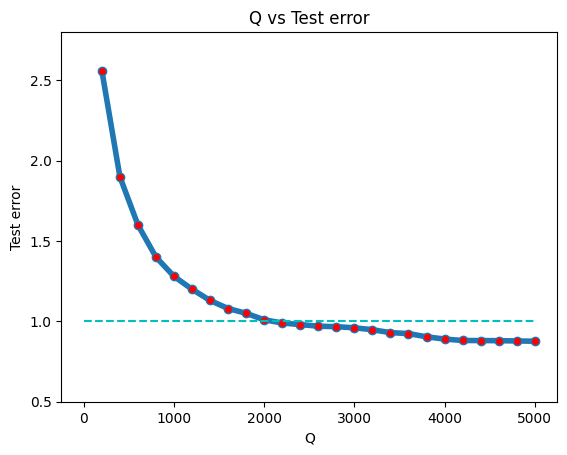
\includegraphics[scale=0.6]{output.png} % Adjust the width as needed
            \caption{$Q$ vs $\eta\%$ (test error)}
            \label{fig}
        \end{figure}

    From the Fig.~\ref{fig} optimal $Q$ was considered as $4000$ where the test error, $\eta = 0.89\%$.

    \section{Conclusion}\label{sec:conclusion}
    First we have used KMeans clustering algorithm to extract a set of representative vectors for each class.
    Then we have passed these representative vectors into LS-SVM kernel model as training dataset.
    This way we have reduced the time complexity of LS-SVM from $O(N^3)$ to $O((KQ)^3)$ where $K$ is the number of classes and $Q$ is number of centroids in each class.
    This method is significantly faster than LS-SVM, it is more robust and easy to implement.

\end{document}
